\documentclass{beamer}
\usepackage[utf8]{inputenc}
\usecolortheme{beaver}
\usepackage{graphicx}
\usetheme{CambridgeUS}
\newcommand\tab[1][1cm]{\hspace*{#1}}


%Information to be included in the title page:
\title{Recreational Marijuana on Traffic Fatalities}
\author{Nhat Hoang Pham	}
\institute{UC Denver}
\date{\today}



\begin{document}

\frame{\titlepage}

\begin{frame} % Slide 1
\frametitle{Research Question}
	What is the effect of Recreational Marijuana Legalization (RML)  on Traffic Fatalities at the state level? 
\end{frame} 

\begin{frame} % Slide 2
\frametitle{Literature Review}
	\begin{itemize}
	
		\item 
		Hansen, Benjamin, Keaton Miller, and Caroline Weber. 2020a. “Early Evidence on Recreational Marijuana Legalization and Traffic Fatalities.” Economic Inquiry, 58(2): 547-568. \pause
		
		\item
		Santaella-Tenorio, Julian, Katherine Wheeler-Martin, Charles J. DiMaggio, Alvaro Castillo-Carniglia, Katherine M. Keyes, Deborah Hasin, and Magdalena Cerdá. 2020. “Association of Recreational Cannabis Laws in Colorado and Washington State with Changes in Traffic Fatalities, 2005-2017.” JAMA Internal Medicine, 180(8): 1061-1068. \pause
		
		\item
		Aydelotte, Jayson D., Lawrence H. Brown, Kevin M. Luftman, Alexandra L. Mardock, Pedro G. R. Teixeira, Ben Coopwood, and Carlos V. R. Brown. 2017. “Crash Fatality Rates After Recreational Marijuana Legalization in Washington and Colorado.” American Journal of Public Health, 107(8): 1329- 1331. \pause
		
	\end{itemize}
\end{frame} 

\begin{frame} % Slide 3
\frametitle{Data at State-Year Level(2010-2019)}
	\begin{itemize}
	
		\item
		FARS from 2010-2019 using accident, accident auxiliary, and person data files
		\item
		U.S census: population, median age, male/female population
		\item
		BEA: Income by state
		\item
		BLS: Unemployment Rate
		\item
		Highway statistics: Number of licensed driver, Vehicle miles driven 		
		\item
		Still working on Drug Per Se Law, Seat Belt Law, Texting Law, Beer Tax etc. 
		
	\end{itemize}
\end{frame} 

\begin{frame} % Slide 4
\frametitle{Variables}

	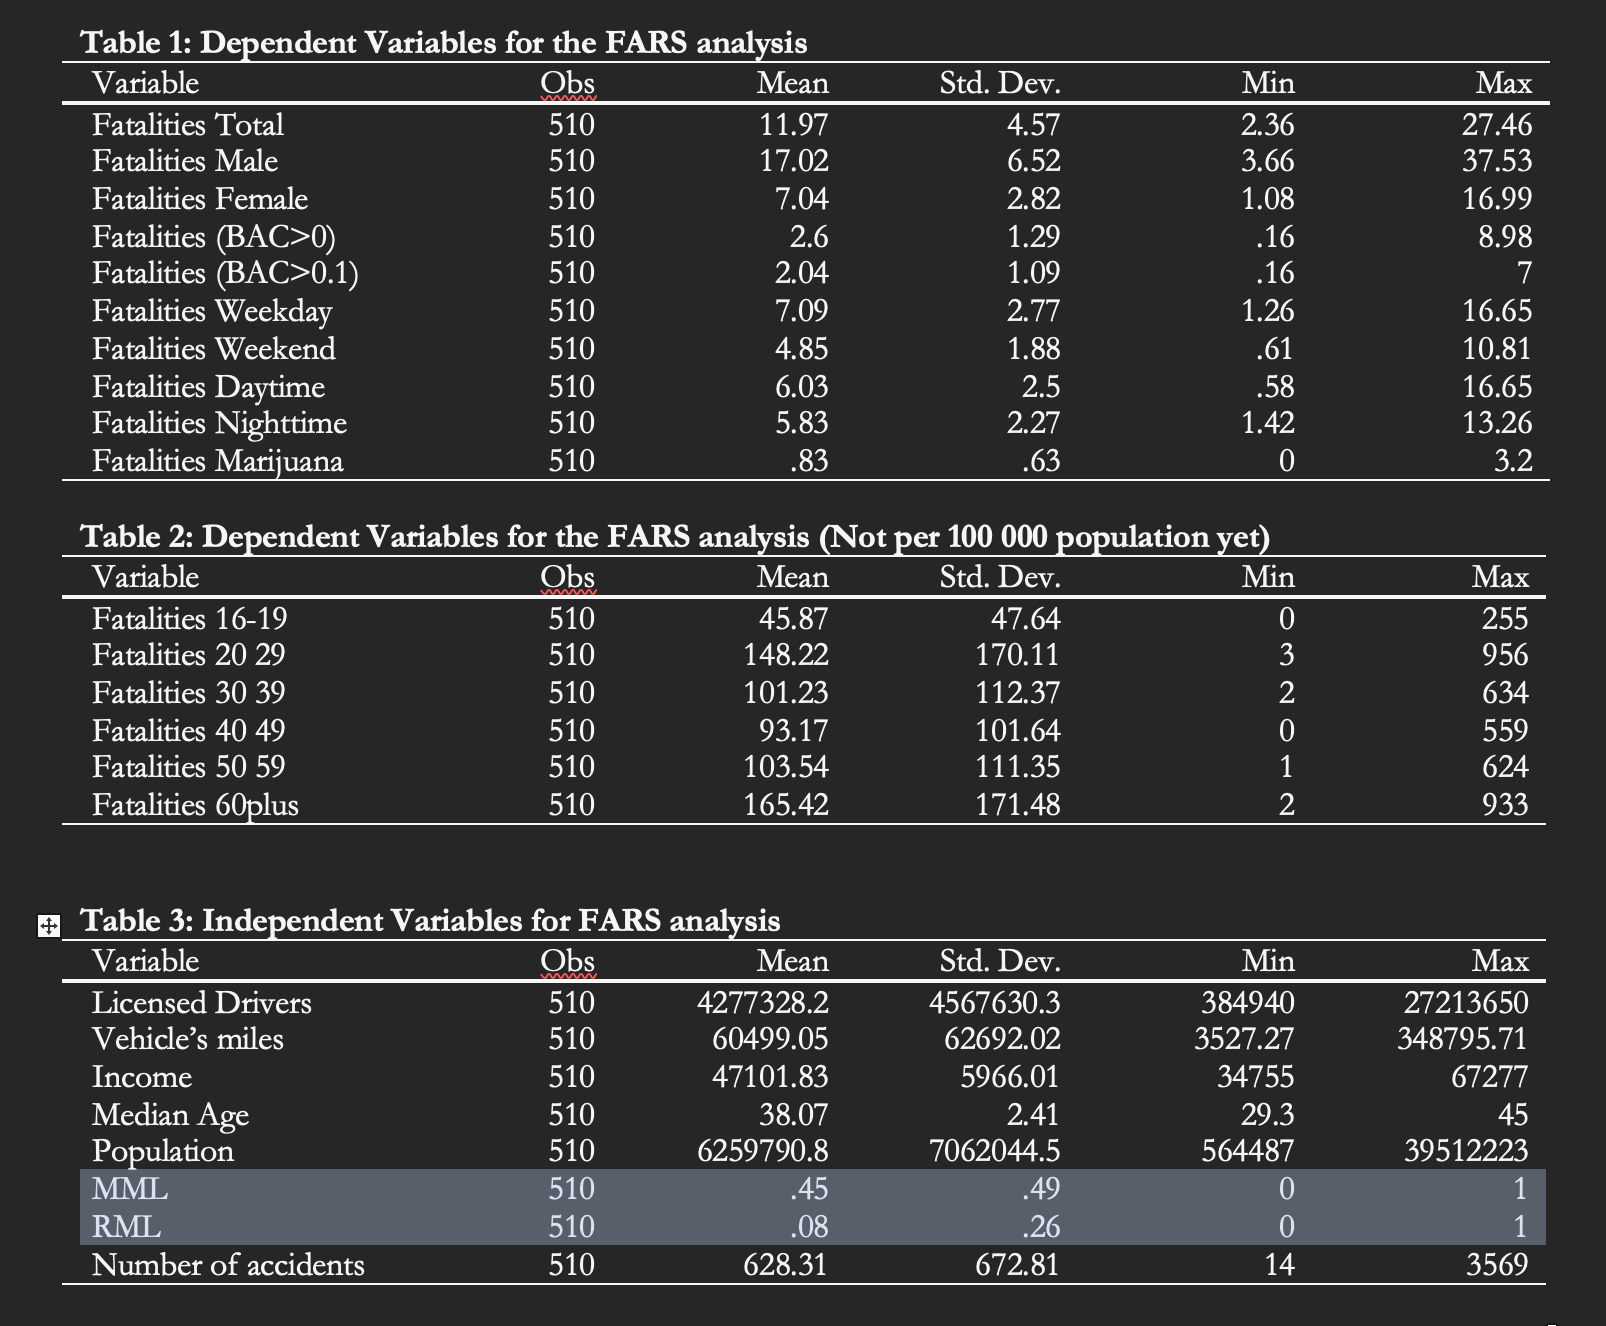
\includegraphics[scale = 0.33]{table123}

\end{frame}

\begin{frame} %Slide 5
\frametitle{Hypothesis}

	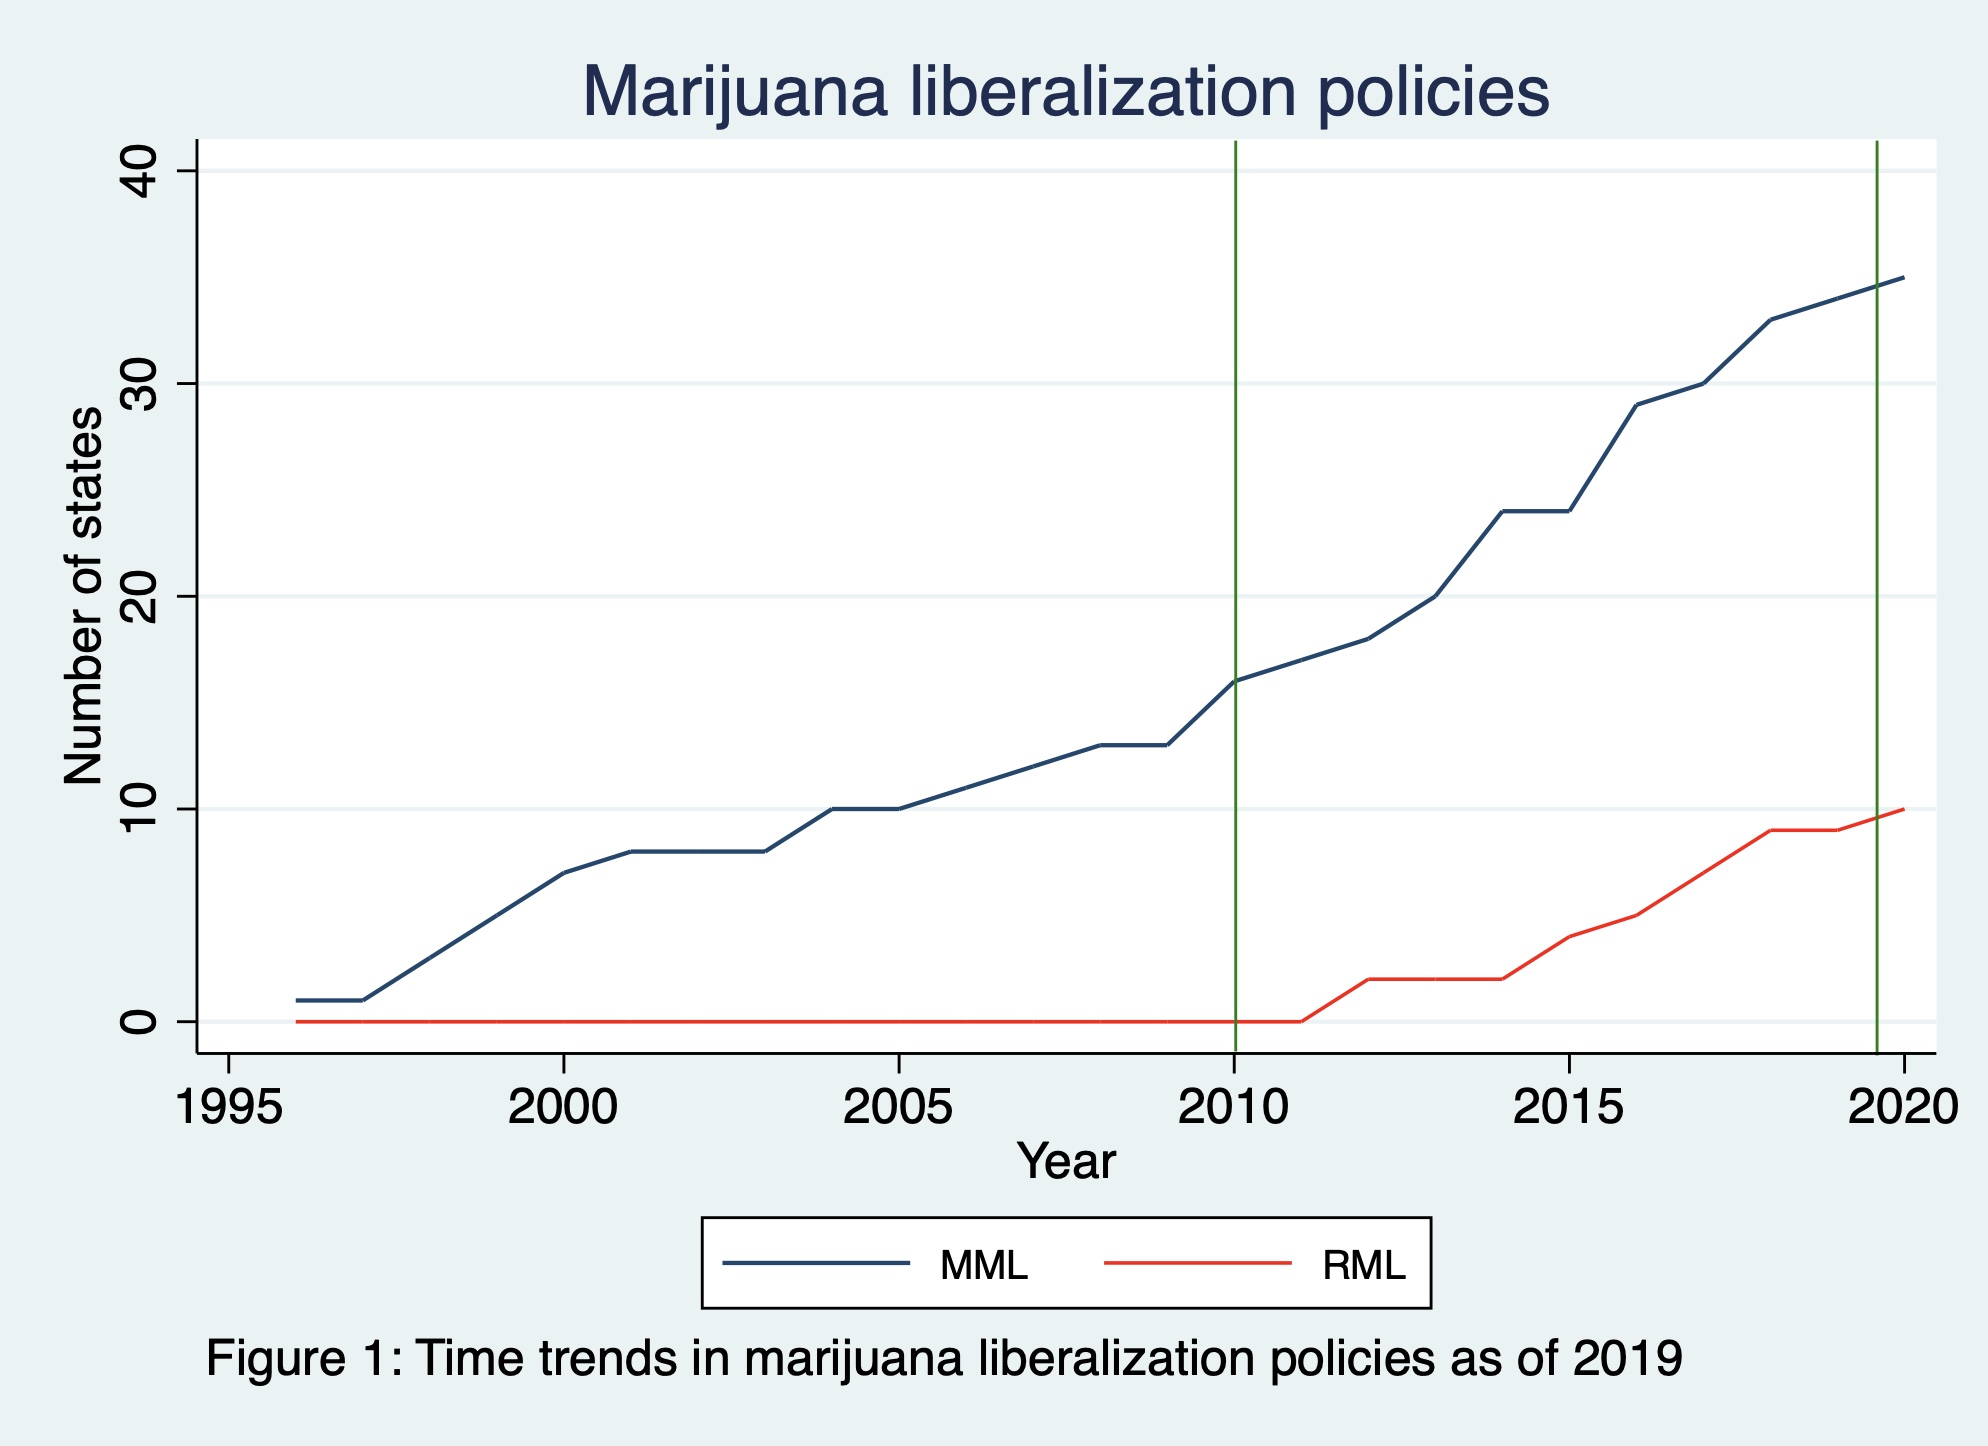
\includegraphics[scale = 0.08]{fig_1.jpg} \\
	Whether RML decrease or increase total traffic fatality, and traffic fatalities involving alcohol, involving marijuana,  different age groups, time of day, day of week.
	
\end{frame}

\begin{frame}
\frametitle{Regression Model}

$$ ln(traffic fatalities_{st}) = \beta_0 + \beta_1 MML + \alert{\beta_2} RML + X_{st} \beta_3 + \mu_s + \eta_t  +\Phi_s *t +\epsilon_{st}$$
Replace MML, RML by MMD, RMD


\end{frame}

\begin{frame} {Potential Robustness Checks}
\begin{itemize}

	\item Dependent variables transformation. (fatalities per licensed driver population, fatalities per vehicle miles traveled, logistic model $ln\frac{fatal}{1- fatal} )$
	
	\item Synthetic control
	
	\item Sample restricted to RML state and neighbor states
	
	\item Different statistical inference for clustered data (cluster-robust variance matrix estimator(standard method), wild cluster bootstrap, DID\_MULTIPLEGT stata module )
\end{itemize}


\end{frame}

\begin{frame}
\frametitle{Note}
Sun and Abraham (2020) have shown that the coefficients in the second regression are not robust to heterogeneous treatment effects across groups and over time,1 and could be misleading even under an additive dynamic treatment effect model with constant effects.  https://arxiv.org/pdf/2007.04267.pdf  \\
https://ideas.repec.org/c/boc/bocode/s458643.html \\ 

Dynamic effects vs instantaneous effect

\end{frame}

\end{document}












